% Definition of radii
\def\firstradius{(0,0) circle (1.5cm)}
\def\secondradius{(1,0) circle (1.5cm)}
\def\thirdradius{(2,0) circle (1.5cm)}

\colorlet{circle edge}{black!100}
\colorlet{circle area}{gray!20}
\tikzset{
  filled/.style={fill=circle area, draw=circle edge, thick},
  outline/.style={draw=circle edge, thick},
  strong/.style={draw=circle edge, ultra thick},
  dash/.style={very thick, dashed}
}

\tikzstyle{vertex}=[circle,fill=black!25,minimum size=10pt,inner sep=0pt]

\setlength{\parskip}{5mm}
 
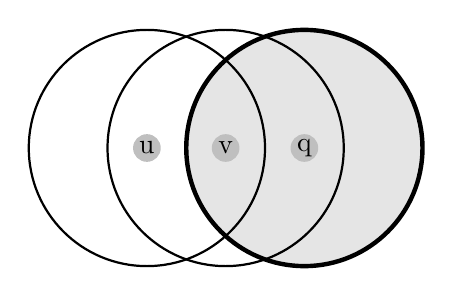
\begin{tikzpicture}
  \node[vertex] (a) at (0,0) {u};
  
  \begin{scope}
    \fill[filled] \thirdradius;
  \end{scope}
   
   % Has to be defined here, or it will be overwritten 
  \node[vertex] (b) at (1,0) {v};
  \node[vertex] (c) at (2,0) {q};   

  \draw[outline] \firstradius node {};
  \draw[outline] \secondradius node {};
  \draw[strong] \thirdradius node {};

\end{tikzpicture}
